\section*{Appendix}
\addcontentsline{toc}{section}{Appendix}

{ \bf Estimation of Yield Curve with Nelson-Siegel-Svensson Model}

\noindent In their seminal paper, \citet{nelson1987parsimonious} specifies the forward rate curve $\tau(f)$ as follows:

\begin{equation}\notag
    f(\tau)=
    \begin{pmatrix}
    \beta_0 \\ \beta_1 \\ \beta_2    
    \end{pmatrix}'
    \begin{pmatrix}
        1 \\ e^{-\tau/\lambda} \\ (\tau / \lambda) e^{-\tau/\lambda}
    \end{pmatrix}
    =
    \begin{pmatrix}
    \beta_0 \\ \beta_1 \\ \beta_2   
    \end{pmatrix}'
    \begin{pmatrix}
    f_0 \\ f_1 \\ f_2  
    \end{pmatrix}
\end{equation}


% Ridge reg paper'ından aynen aldım
\noindent The spot rate function, which is the average of the forward rate curve up to time to maturity $\tau$, is defined as:

\begin{equation}\notag
    r(\tau)= \frac{1}{\tau}\int_0^\tau f(u)\,du
\end{equation}

\noindent with continuous compounding. Hence, the corresponding spot rate function at time to maturity $\tau$ reads

\newpage

\noindent { \bf Historical Interest Rates}

\begin{figure}[H]
    \centering
    \caption{Long-Term \textit{Nominal} Interest Rates}
    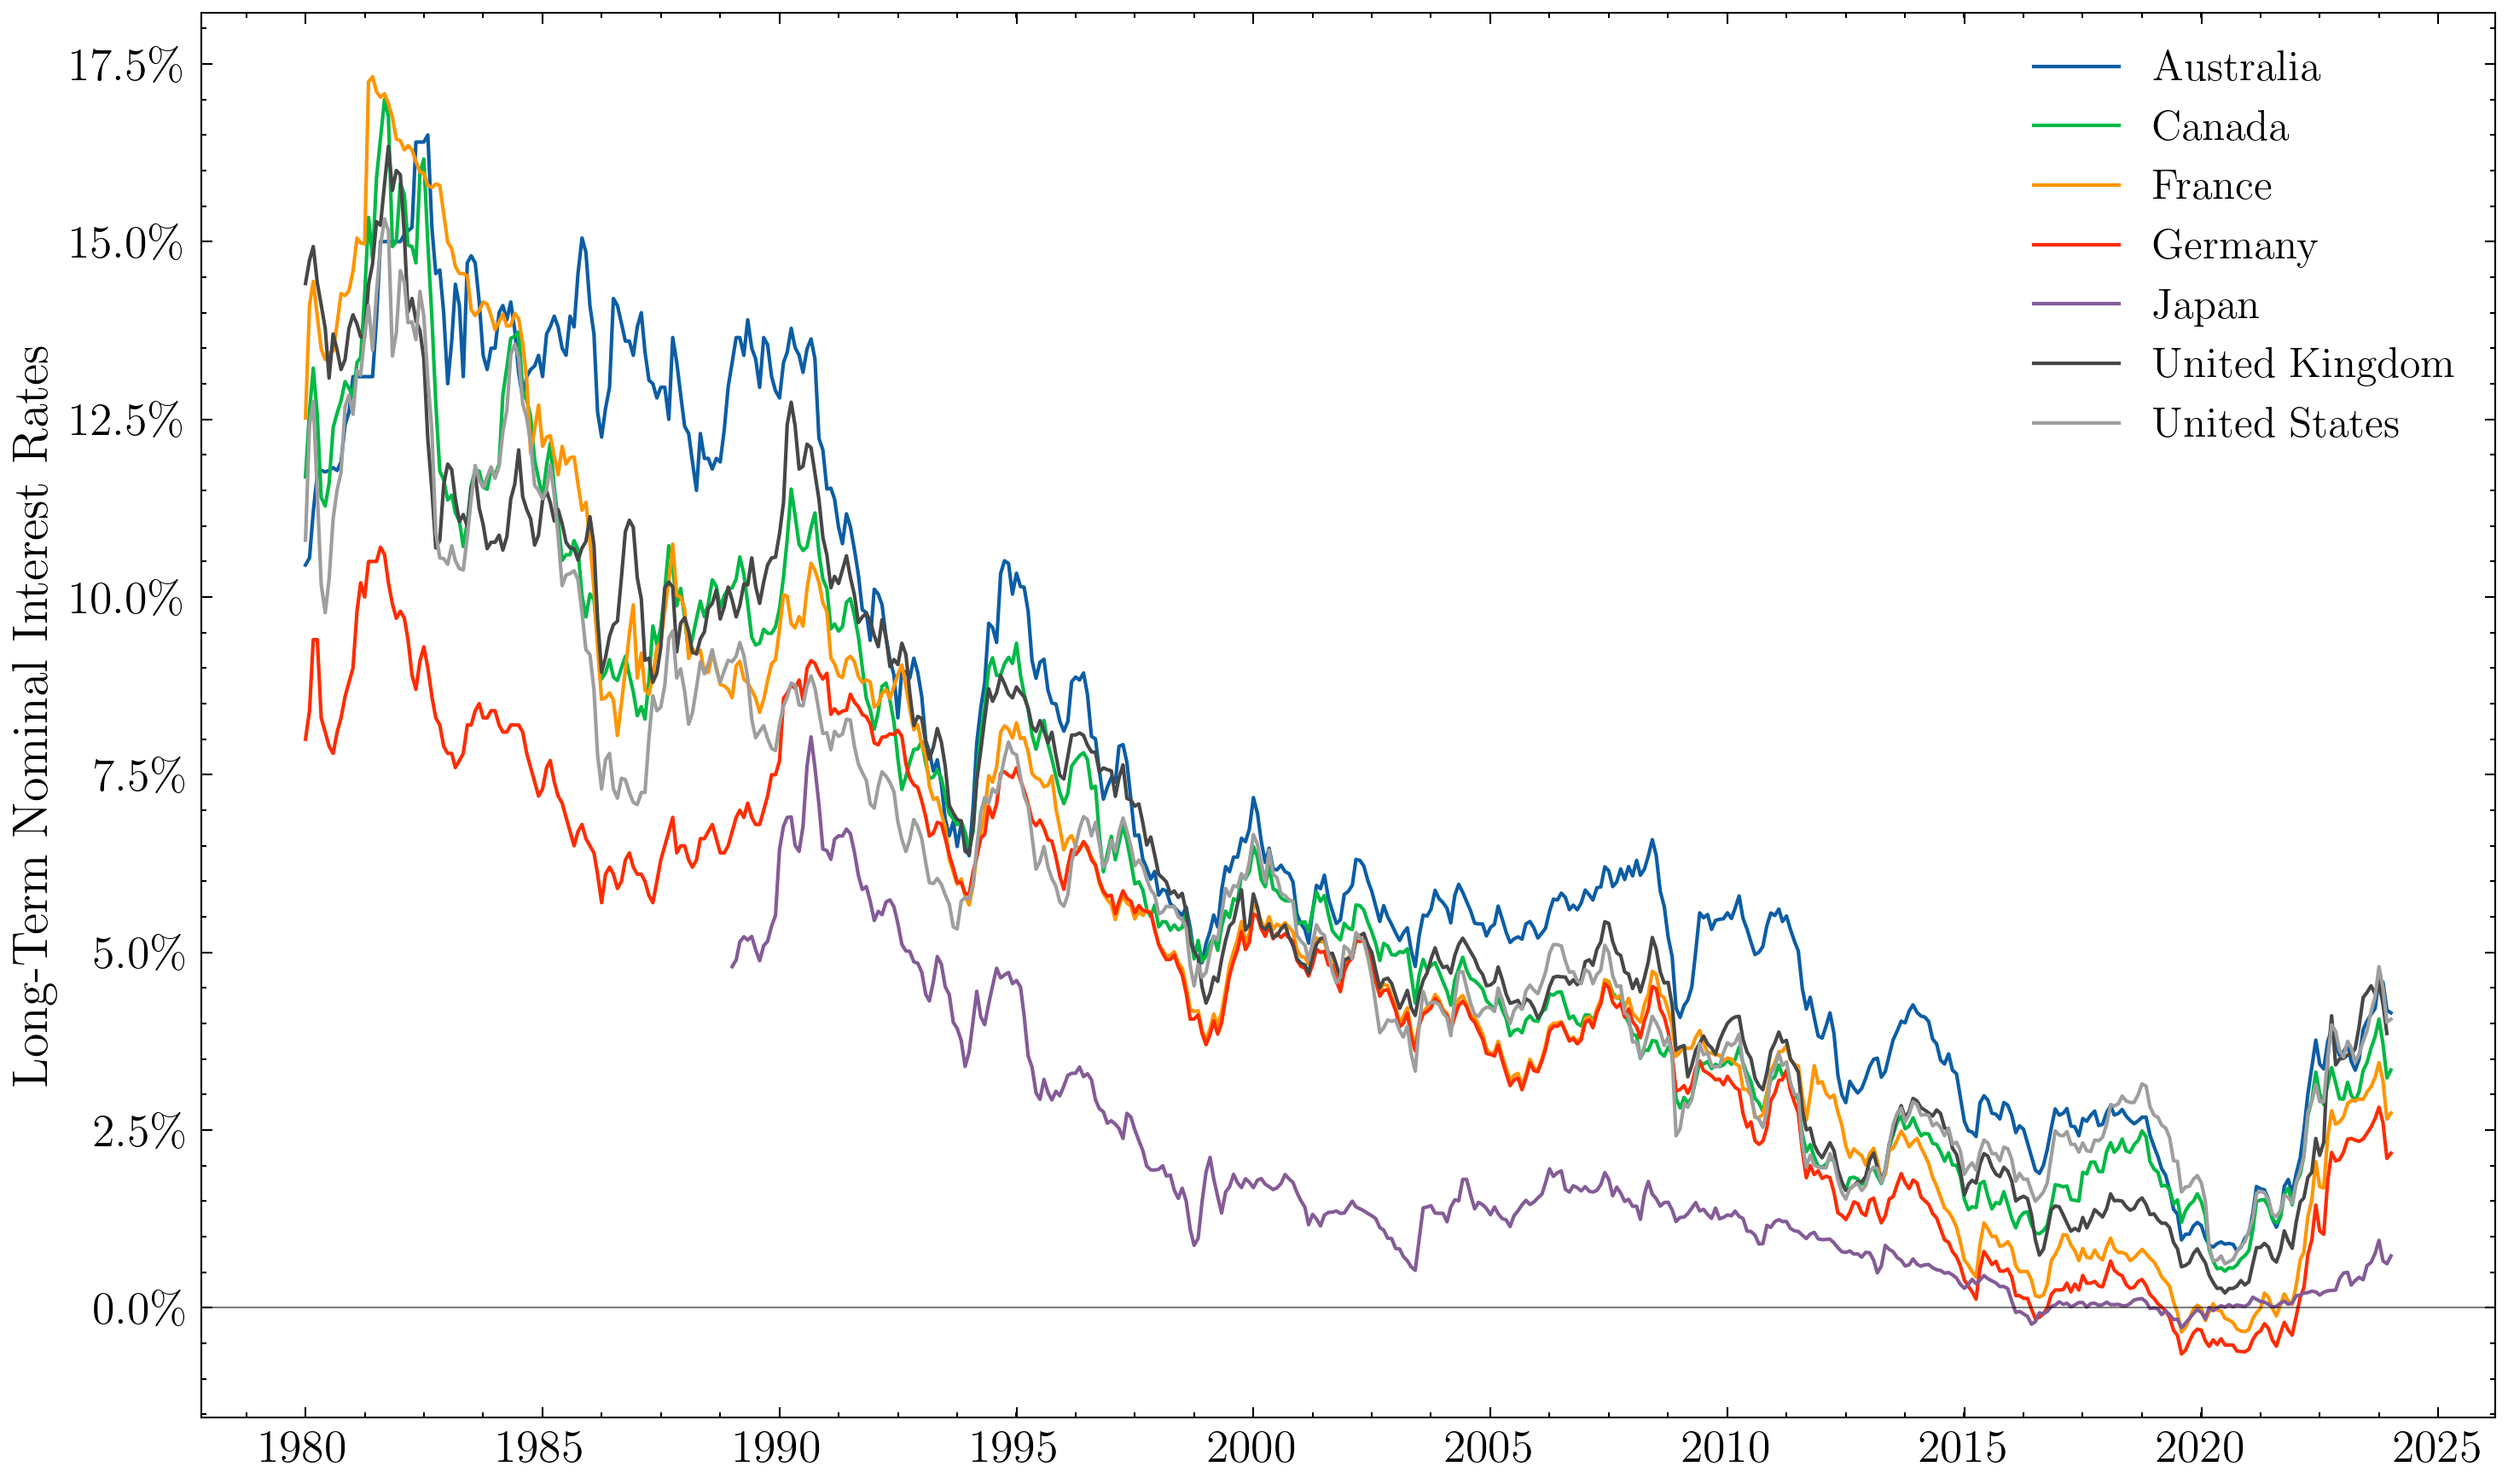
\includegraphics[width=0.8\textwidth]{figures/long-term-rates.png}
    
    \vspace{15pt}
    
    \begin{minipage}{\textwidth}
        \footnotesize % Adjust font size to 8pt
        \textbf{Note:} In this figure, long-term interest rates refer to 10-year bond yields. The data is obtained from OECD Database.
    \end{minipage}
    \label{fig:long-term-rates}
\end{figure}

\begin{figure}[H]
    \centering
    \caption{Yield Curves of Sampled Countries}
    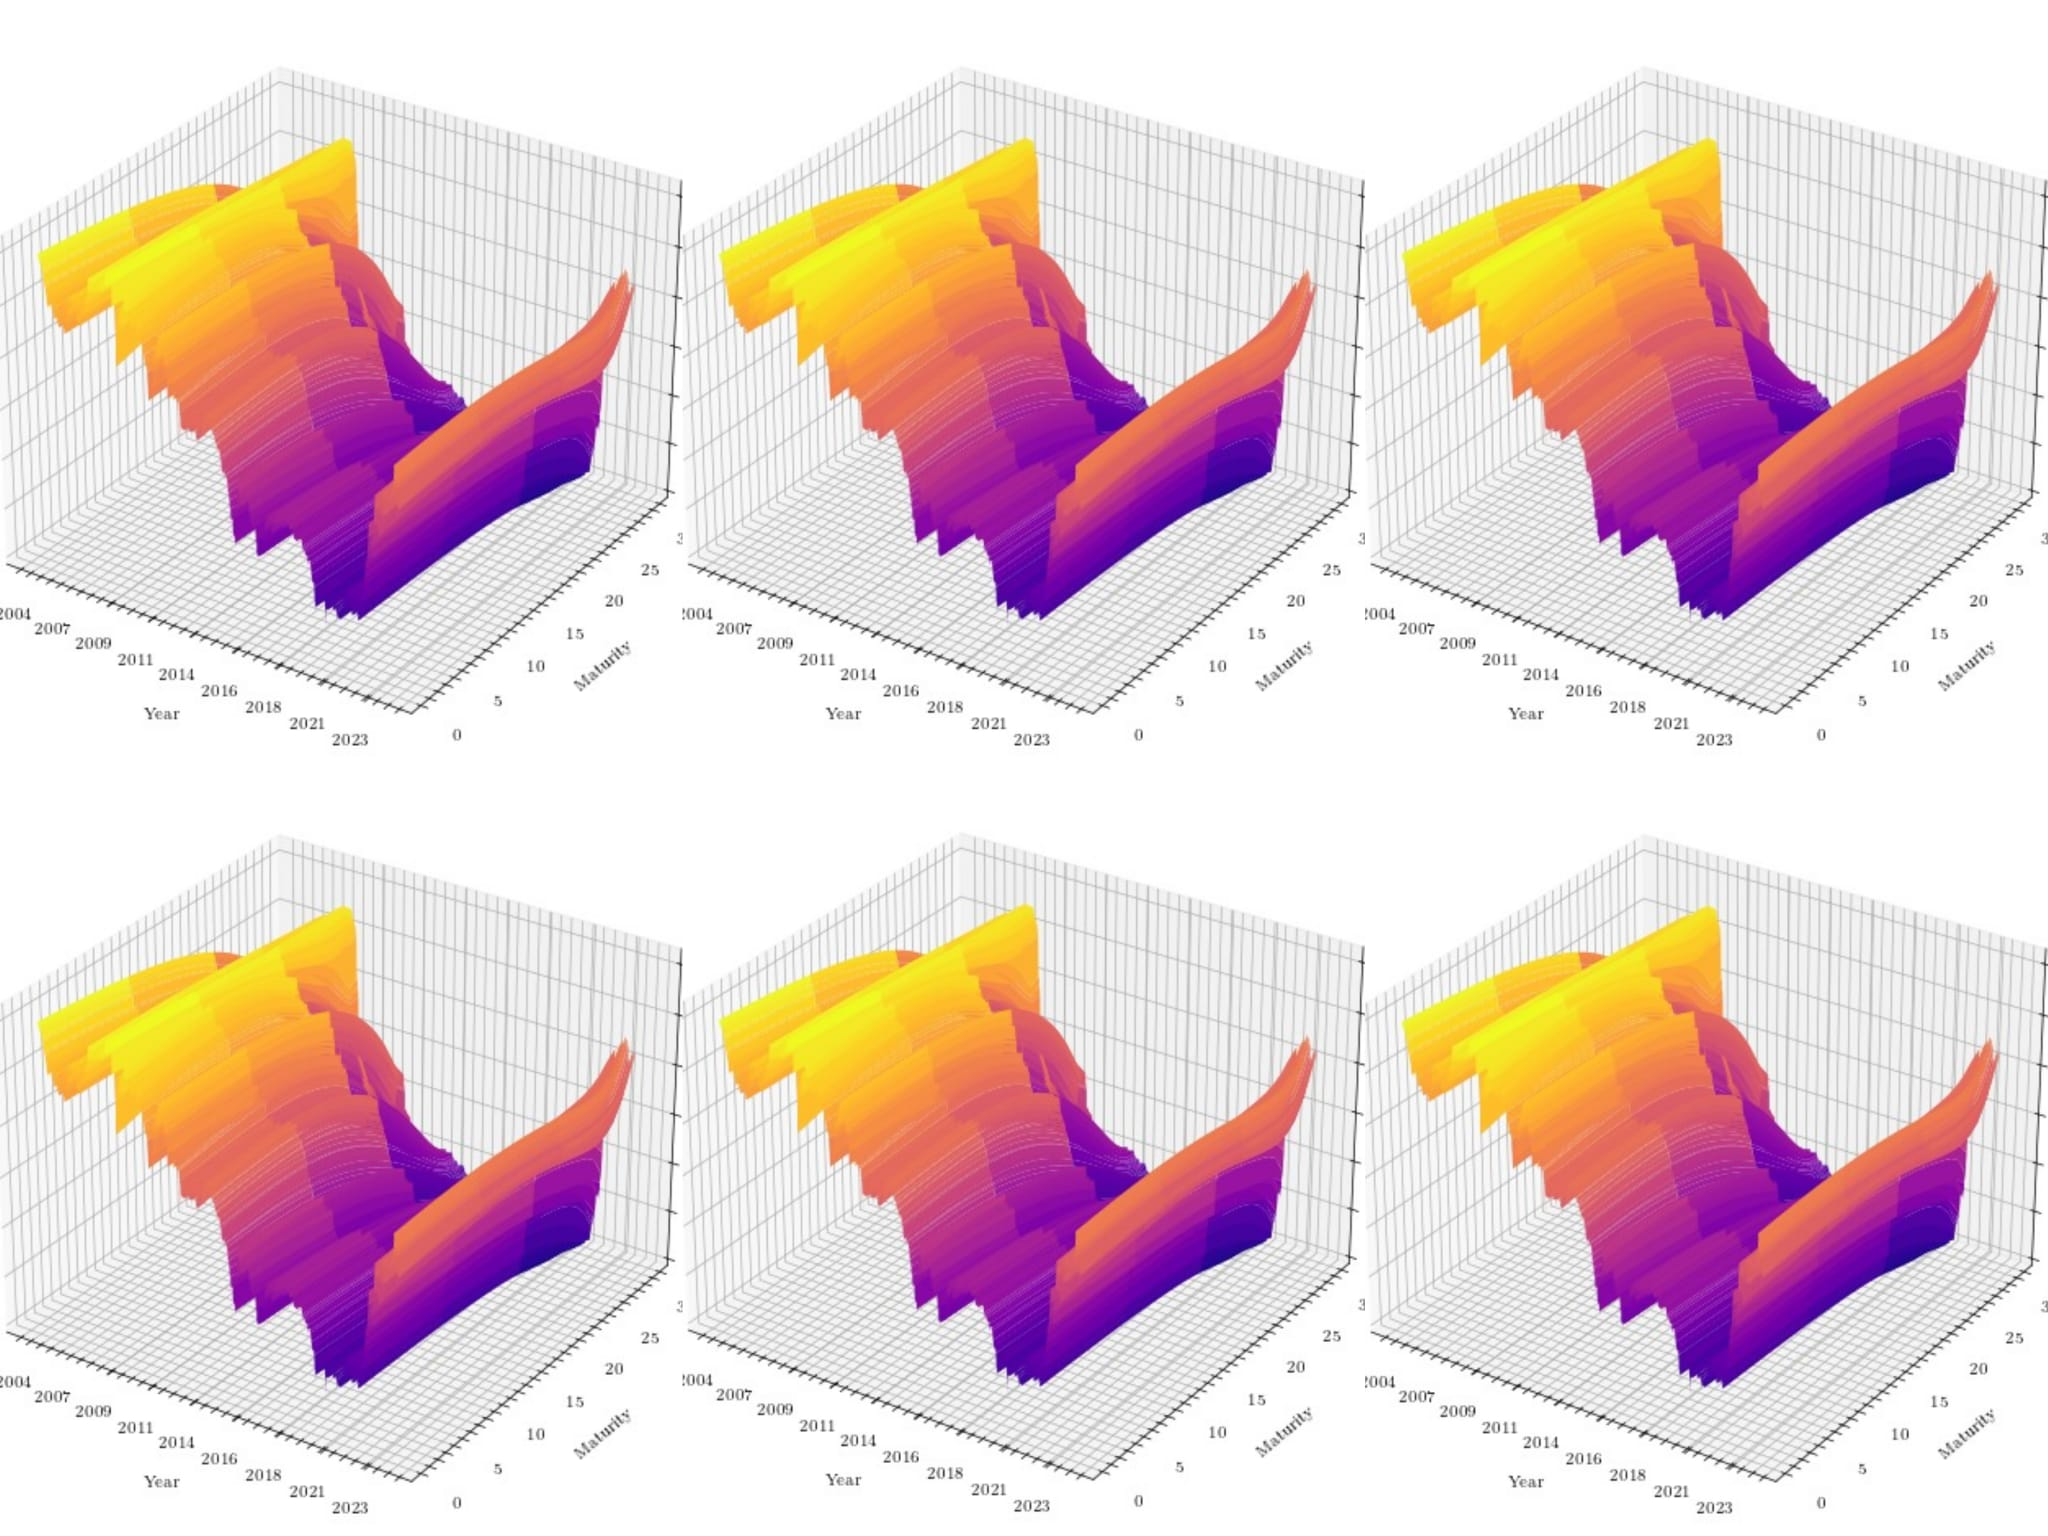
\includegraphics[width=0.9\textwidth]{figures/ycs.jpg}
\end{figure}

\newpage

\begin{table}[!htbp] \centering
  \caption{Regression Results}
\begin{tabular}{@{\extracolsep{5pt}}lccccc}
\\[-1.8ex]\hline
\hline \\[-1.8ex]
& \multicolumn{5}{c}{\textit{Dependent variable: 10yr Change}} \
\cr \cline{2-6}
\\[-1.8ex] & \multicolumn{1}{c}{ECB} & \multicolumn{1}{c}{BoE} & \multicolumn{1}{c}{BoJ} & \multicolumn{1}{c}{SNB} & \multicolumn{1}{c}{RBA}  \\
\hline \\[-1.8ex]
 In BoE 3dWindow & & -0.003$^{}$ & & & \\
& & (0.006) & & & \\
 In BoJ 3dWindow & & & 0.000$^{}$ & & \\
& & & (0.001) & & \\
 In ECB 3dWindow & 0.000$^{}$ & & & & \\
& (0.002) & & & & \\
 In Fed 3dWindow & -0.003$^{}$ & -0.013$^{**}$ & -0.003$^{***}$ & 0.001$^{}$ & -0.004$^{}$ \\
& (0.002) & (0.006) & (0.001) & (0.002) & (0.003) \\
 In RBA 3dWindow & & & & & -0.001$^{}$ \\
& & & & & (0.005) \\
 In SNB 3dWindow & & & & -0.001$^{}$ & \\
& & & & (0.002) & \\
 Intercept & -0.000$^{}$ & 0.004$^{**}$ & 0.000$^{}$ & -0.001$^{}$ & -0.001$^{}$ \\
& (0.001) & (0.002) & (0.000) & (0.000) & (0.001) \\
\hline \\[-1.8ex]
 Observations & 5005 & 1263 & 4010 & 6324 & 5275 \\
 $R^2$ & 0.000 & 0.005 & 0.002 & 0.000 & 0.000 \\
 Adjusted $R^2$ & 0.000 & 0.003 & 0.002 & -0.000 & -0.000 \\
 Residual Std. Error & 0.041 & 0.058 & 0.019 & 0.034 & 0.074 \\
 F Statistic & 1.151$^{}$ & 2.978$^{*}$ & 4.700$^{***}$ & 0.192$^{}$ & 0.686$^{}$ \\
\hline
\hline \\[-1.8ex]
\textit{Note:} & \multicolumn{5}{r}{$^{*}$p$<$0.1; $^{**}$p$<$0.05; $^{***}$p$<$0.01} \\
\end{tabular}
\end{table}